% -*- root: ../../main.tex -*-
%!TEX root = ../../main.tex
% this file is called up by main.tex
% content in this file will be fed into the main document
% vim:textwidth=80 fo=cqt

At this  stage, it must  be recalled that the  purpose of developing  the system
identification electrolyte  model was  to mitigate the  poor performance  of the
basic  \gls{spm} at  C-rates above~0.5C (see \cref{subsec:simresultsbasicspm}).
This sub-optimal performance was attributed  to the lack of electrolyte dynamics
in  the  basic  \gls{spm}.  The   performance  of  the  newly  developed  system
identification model has been proved to be  superior to the current state of the
art. The next step  is to embed this electrolyte model  into the basic \gls{spm}
so as to  obtain a composite \gls{spm}. The performance  of this composite model
is evaluated to ascertain its suitability towards online implementation.

\subsection{Computation of electrolyte overpotential}\label{subsec:electrolyteopcalc}

The missing component in the terminal voltage computation of the basic \gls{spm}
is  the  contribution from  the  electrolyte  overpotential  term. This  is  the
potential difference in  the entire electrolyte \ie~the electrolyte potential
at the positive current collector interface with respect to that at the negative
current collector interface.


As discussed in \cref{sec:electrolyteinclusion}, using  the equation proposed by
Prada~\etal~\cite{Prada2012}, the  overpotential in the electrolyte  is computed
as
\begin{align}
    \quad \phi_\epos - \phi_\eneg &= (1-t_{+}^0) \frac{2RT}{F}\ln \frac{c_\text{e,\tiny pos/cc}}{c_\text{e,\tiny neg/cc}}\nonumber\\
    {} &\quad -\frac{I}{2 A}\left(\frac{l_\text{neg}}{\kappa_\text{eff,neg}} + 2 \frac{l_\text{sep}}{\kappa_\text{eff,sep}} + \frac{l_\text{pos}}{\kappa_\text{eff,pos}}\right) \tag{\cref{eq:electrolytepdwithce} revisited}
\end{align}

\Cref{eq:electrolytepdwithce} consists of two distinct terms ---
\begin{enumerate*}[label=\roman*)]
    \item a diffusion overpotential due to concentration gradient in the electrolyte, and
    \item an ohmic resistance term that is dependent upon
        \begin{enumerate*}[label=\itshape\alph*\upshape)]
            \item the instantaneous value of applied current,
            \item the thicknesses of the three cell regions, and
            \item the effective ionic conductivity in each of the three regions. %which in-turn depends on ionic concentration,.
        \end{enumerate*}
\end{enumerate*}

The ohmic  loss term  of \cref{eq:electrolytepdwithce} needs  to be  examined in
closer detail.  The dependence of  this term  on instantaneous load  current and
cell thicknesses  can be accounted  in a straightforward manner.  However, there
are ambiguities  in computing the  effective ionic  conductivity in each  of the
three cell regions. The effective value of ionic conductivity in the electrolyte
depends on its intrinsic conductivity, the Bruggeman constants and porosities of
each  of  the three  regions.  The  intrinsic electrolyte  conductivity  in-turn
depends on the electrolyte concentration.

Ambiguities   arise   in  interpreting   the   value   of  ionic   concentration
to   be    used   for   computation   of    electrolyte   concentration.   Since
\cref{eq:electrolytepdwithce}  deals  with  overall potential  drop  across  the
entire  length of  the cell,  the concentration  used for  computing electrolyte
conductivity could,  for example be  that at the respective  current collectors.
This concept however  introduces inconsistencies with the  separator term. Using
the  separator concentration  from one  of the  electrode interfaces  introduces
unequal  weighting  in this  computation.  If  the  ionic concentration  at  the
midpoint of the separator is used, this scheme becomes inconsistent with that at
the  two current  collectors. Another  possibility for  computing the  effective
conductivity in a  cell region is to  use the mean of the  concentration in that
region. However, since the mean is nothing but a simple statistical first moment
is  equally influenced  by the  entire  concentration profile  within each  cell
region. This is questionable given that the electrolyte overpotential across the
entire cell thickness  is most likely governed by the  conductivities at the two
current  collector interfaces.  Some form  of weighted  mean could  be conjured,
wherein the  current collector locations  are given  the highest weight  and the
separator locations the  least weight. However, finding the  weights becomes yet
another  exercise and  from the  engineering perspective  of computing  these in
real-time, seems to be in the realm of diminishing returns.

In  published  literature,  only  a  cursory  treatment  has  been  accorded  to
the  aforementioned  ambiguities.  In  Prada~\etal~\cite{Prada2012},  the  usage
of  initial concentrations  is  used  to only  introduce  the  concept of  ohmic
resistance  in that  article.  However,  the author  of  this  thesis wishes  to
extend  this  concept further.  In  the  simulations  conducted by  this  thesis
author, it  became clear  that the  dependence on  applied current  was required
in  order to  obtain  reasonable accuracies.  Computing  mean of  concentrations
in  cell  regions for  calculation  of  ionic  conductivities  led to  a  biased
computation of overpotentials.  Therefore, this author decided to  use the value
of  initial concentration  for the  computation of  ionic conductivities  in the
current-dependent  contribution  to  electrolyte  overpotential  throughout  the
entire time horizon considered.

Hence, as per the adopted scheme \cref{eq:electrolytepdwithce} gets modified as
\begin{align}
    \quad \phi_\epos(t) - \phi_\eneg(t) & = (1-t_{+}^0) \frac{2RT}{F}\ln \frac{c_\text{e,\tiny pos/cc}(t)}{c_\text{e,\tiny neg/cc}(t)}\nonumber \\
    {}                             &\quad -\frac{I}{2 A}\left(\frac{l_\text{neg}}{\kappa_\text{eff,neg}\left(c_\text{e}\left(0\right)\right)} + 2
    \frac{l_\text{sep}}{\kappa_\text{eff,sep}\left(c_\text{e}\left(0\right)\right)} +
\frac{l_\text{pos}}{\kappa_\text{eff,pos}\left(c_\text{e}\left(0\right)\right)}\right)\label{eq:electrolytepdwithcenew}
\end{align}
wherein  the time-dependent terms are explicitly shown in the notation.

Using \cref{eq:electrolytepdwithcenew} for electrolyte overpotential computation
has an  important implication. The  two-pronged influence of  the time-dependent
electrolyte concentration on the electrolyte overpotential \viz
\begin{enumerate*}[label=\itshape\alph*\upshape)]
    \item a direct influence in the form of concentration dependent diffusion polarisation, and
    \item an indirect influence through its use in ionic conductivity calculations
\end{enumerate*}
has  now  been  reduced  to  just   one.  This  implies  the  results  from  the
system  identification   model  are  now   required  only  in  the   first  term
of \cref{eq:electrolytepdwithcenew}.

In the light of the decision of use the (constant) initial concentration for the
ohmic term, it is natural to question the gains from the circuitous route of the
system  identification  exercise that  was  undertaken  to obtain  the  improved
electrolyte model. Therefore,  it is imperative to quantify  the relative weight
of  the  concentration  dependent  diffusion resistance  compared  to  the  bulk
solution resistance.

\begin{figure}[!htbp]
    \centering
    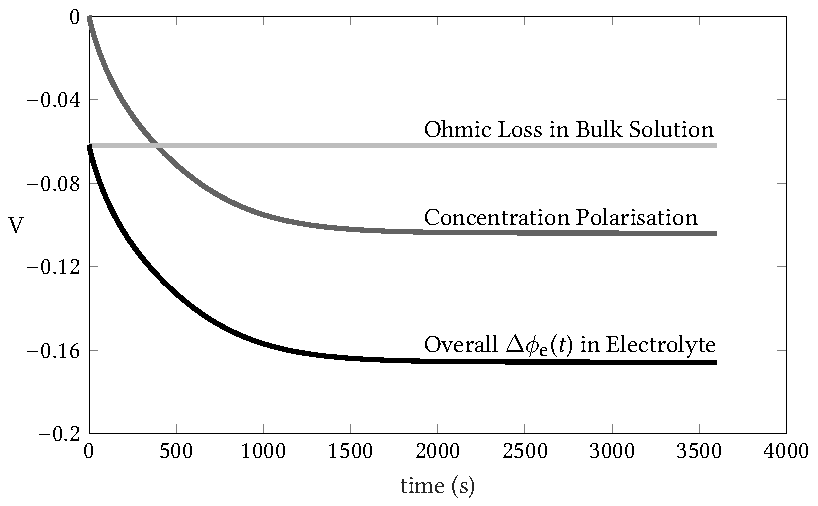
\includegraphics{contribution_to_phie_1C.pdf}
    \caption[%
    Contribution to electrolyte overpotential from the gradient-induced polarisation
    term and the bulk solution resistance term for a 1C~discharge
    ]%
    {%
        Contribution to the overpotential in the electrolyte from each of the
        two terms in \cref{eq:electrolytepdwithcenew} for a 1C~discharge. The
        bulk solution resistance is approximated as a constant value determined
        by the equilibrium initial concentration. The concentration dependent
        polarisation term governs the dynamic behaviour of the overall
        overpotential. Furthermore, this gradient-induced diffusion resistance
        has a strong contribution to the steady state, higher than the bulk
        solution resistance and cannot be neglected without introducing
        significant errors.
}%
\label{fig:contributiontophiefromtwoterms}
\end{figure}

\Cref{fig:contributiontophiefromtwoterms} shows the  contribution to the overall
potential drop~$\phi_\text{e,pos}$ and~$\phi_\text{e,neg}$ in  the electrolyte
from  each  of  the  two  terms  in \cref{eq:electrolytepdwithcenew}  for  a  1C~discharge. The bulk  solution resistance is constant owing to  the fact that the
initial  electrolyte concentration  is  used in  computing  the effective  ionic
conductivities in the three regions of  the cell. The gradient induced diffusion
polarisation term, however has a stronger contribution in both the transient and
steady  state. The  entire dynamics  of the  overall potential  drop during  the
transient  phase is  governed by  this concentration-dependent  term, while  its
steady state contribution  is in-fact higher than the  bulk solution resistance.
The  constant  ohmic resistance  term  merely  provides  a non-zero  offset  for
the  electrolyte  solution  overpotential.  In questioning  whether  the  system
identification exercise was indeed worthwhile,  if the concentrations in the two
current collectors had not been computed  at each time-step, then this diffusion
polarisation  term  would  become  zero.  This is  because,  the  numerator  and
denominator in \cref{eq:electrolytepdwithcenew} would have to be retained at the
initial concentration, leading to a unit  ratio whose natural logarithm is zero.
Therefore, it  is clear  that computing  the concentrations  at the  two current
collectors  through system  identification has  indeed helped  in improving  the
modelling accuracy.

Having established the relative  importance of computing the diffusion-dependent
polarisation   overpotential,  the   next  question   that  arises   is  whether
the   constant    approximation   for   the   bulk    solution   resistance   is
indeed   appropriate.   It  also   remains   to   be   seen  if   the   accurate
computation   of  the   ionic   concentration   through  system   identification
(see \cref{sec:perfanalysisnewmodel}) has  translated into a  similarly accurate
computation of  electrolyte overpotential. This  is answered by a  comparing the
electrolyte overpotential computed by the  system identification model with that
obtained from the \gls{p2d} model.

\begin{figure}[!htbp]
    \centering
    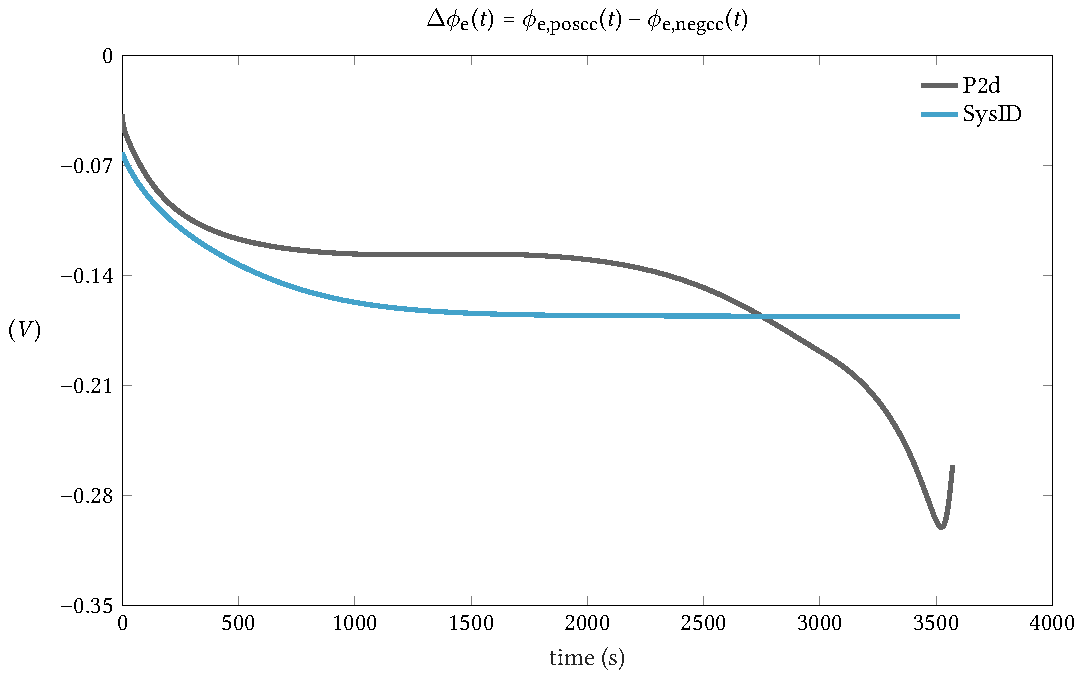
\includegraphics{phie_delta_cnst_1C.pdf}
    \caption[%
    Electrolyte  overpotential  computed  by the  \glsfmtshort{p2d}  and  system
    identification models for a 1C~discharge
    ]%
    {%
        Comparison    of    electrolyte    overpotential   computed    by    the
        \gls{p2d}     model    and     the    system     identification    model
        (using \cref{eq:electrolytepdwithcenew}) for a  1C~discharge. During the
        transient phase, the profile obtained by the system identification model
        closely matches that of the \gls{p2d} model. The mismatch in the initial
        overpotential does not arise to the  use of a constant concentration for
        the bulk  resistance contribution,  since at  equilibrium this  value is
        exact and  not an  approximation. Past  the initial  transient, accuracy
        of  the system  identification  model degrades.  This  can be  explained
        by  its  analogous  behaviour   for  concentration  computation  in  the
        \glsfmtlong{qss} (see \cref{subsec:tfquadceconstcurrinput}) for constant
        current inputs.
    }%
    \label{fig:phiedeltacnst1C}
\end{figure}

\Cref{fig:phiedeltacnst1C} shows  a comparison of the  electrolyte overpotential
computed  by   the  \gls{p2d}  and   system  identification  models  for   a  1C~discharge. There  is a discrepancy  in the  initial offset of  the overpotential
value.  However,  this  cannot  be  attributed   to  the  use  of  the  constant
concentration  approximation   in  the   computation  of   ionic  conductivities
in \cref{eq:electrolytepdwithcenew}.  This   is  because,  at   equilibrium  the
concentration used  is exactly  the initial  concentration. Furthermore,  at the
instant of applying the current, diffusion gradients in the electrolyte have not
yet been established.  Hence, the contribution from  the diffusion overpotential
is zero,  which can  also be  seen in \cref{fig:contributiontophiefromtwoterms}.
Thus, it can be  concluded that this initial mismatch is due  to the presence of
some  other unmodelled  phenomena  that  affects the  DC  offset of  electrolyte
overpotential, and is not arising due to the approximations used by this author.

In \cref{fig:phiedeltacnst1C},   the  shape   of   the   transient  profile   of
overpotential  computed  by  the  system identification  model  closely  matches
that  of the  \gls{p2d} model.  This validates  that the  newly developed  model
does  indeed  capture the  electrolyte  dynamics  sufficiently well  during  the
initial transient.  However, past  the initial  transient, the  model's accuracy
degrades and  the resulting  profile does  not track  the \gls{p2d}  model. This
behaviour in overpotential is analogous to that exhibited in the spatio-temporal
concentration   study   discussed  in \cref{subsec:tfquadceconstcurrinput}   for
constant current inputs,  wherein it was deemed that this  newly developed model
is  more  suitable  for  dynamic  loads. The  same  conclusion  for  electrolyte
overpotential   accuracy  is   reached   from  this   constant  current   study.
Nevertheless, even for  constant current loads, using the  newly developed model
is better than having no electrolyte model whatsoever as in the basic \gls{spm}.


\begin{figure}[!htbp]
    \centering
    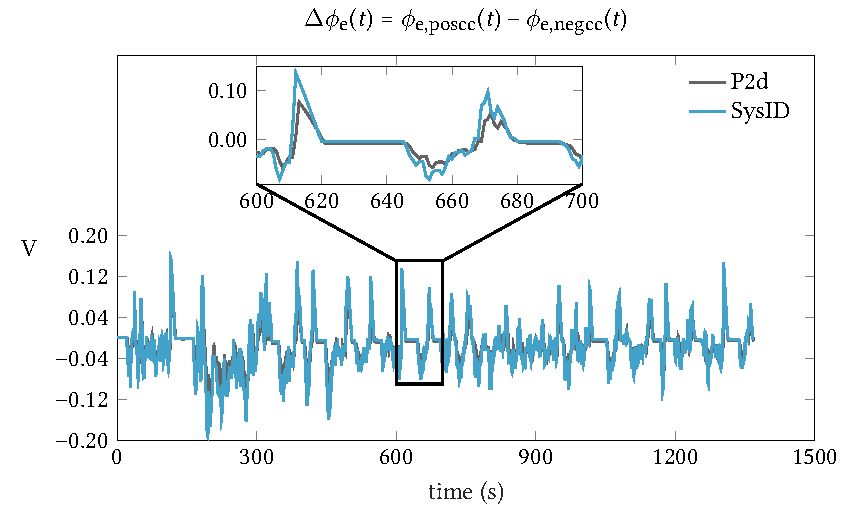
\includegraphics{phie_delta_udds.pdf}
    \caption[%
    Electrolyte  overpotential  computed  by the  \glsfmtshort{p2d}  and  system
    identification models for a \glsfmtshort{udds} load profile
    ]%
    {%
        Comparison    of    electrolyte    overpotential   computed    by    the
        \gls{p2d}     model    and     the    system     identification    model
        (using \cref{eq:electrolytepdwithcenew}) for a  \gls{udds} load profile.
        The overpotential  profile computed  by the system  identification model
        reasonably matches  the profile obtained  by the \gls{p2d} model  with a
        \glsfirst{mae} of \SI{15.88}{\milli\volt} and  a \glsfirst{rms} error of~\SI{24.11}{\milli\volt}.
    }%
    \label{fig:phiedeltacnstudds}
\end{figure}

\Cref{fig:phiedeltacnstudds} shows a comparison of the electrolyte overpotential
computed by the \gls{p2d} and system identification models for a \gls{udds} load
profile. The  input current corresponding to  this load profile is  shown in the
top row  of \cref{fig:uddssimp2dspmresults}. The system  identification model is
able to  reasonably track  the overpotential profile  computed by  the \gls{p2d}
model. Unlike the  case of sustained unidirectional current input,  the error in
this case  remains well-contained. The  \gls{mae} obtained for this  profile was
\SI{15.88}{\milli\volt}  with  an  \gls{rms}  error  of~\SI{24.11}{\milli\volt}.
This  corresponds to  \SI{8.19}{\percent} and  \SI{12.44}{\percent} of  the peak
magnitude of the overpotential (\SI{193.86}{\milli\volt}).

Hence, it can be concluded  that the electrolyte overpotential computation using
the system identification  model provides an acceptable  performance for dynamic
load profiles.  The next step  is to incorporate this  electrolyte overpotential
calculation into the basic \gls{spm} and to quantify the voltage accuracy of the
resulting composite \gls{spm}.

\subsection{Terminal voltage computation of composite \glsfmtshort{spm}}

In \cref{subsec:simresultsbasicspm}, it  was shown that in  the basic \gls{spm},
the computation of the cell's \gls{soc}  is of sufficient accuracy. However, its
terminal  voltage  strongly deviates  from  the  true  value  as computed  by  a
\gls{p2d} model.  This mismatch between  \gls{soc} and terminal  voltage hinders
the  suitability of  the basic  \gls{spm}  as the  plant model  in online  state
estimation applications. The discrepancy in terminal  voltage is due to the lack
of electrolyte overpotential contribution in  its computation. Having obtained a
suitable methodology  to compute this  (see \cref{subsec:electrolyteopcalc}), it
is now possible to refine the computation of the cell's terminal voltage.

Referring   to \cref{eq:posoverpotential}  and \cref{eq:negoverpotential},   the
reaction overpotential in each of the two porous electrode regions is given by
\begin{align}
    η_\text{pos} &= ϕ_\spos - ϕ_\epos - U_\text{pos} \label{eq:posoverpotentialoverall} \\% \tag{\cref{eq:posoverpotential} revisited}\\
    η_\text{neg} &= ϕ_\sneg - ϕ_\eneg - U_\text{neg} \label{eq:negoverpotentialoverall} %\tag{\cref{eq:negoverpotential} revisited}
\end{align}
wherein  the  contribution  from   the  electrolyte  potential  terms~$ϕ_\epos$
and~$ϕ_\eneg$ are no longer to be neglected.

Subtracting \cref{eq:negoverpotentialoverall}
from \cref{eq:posoverpotentialoverall}
\begin{align}
 η_\text{pos} - η_\text{neg} &= \underbrace{ϕ_\spos - ϕ_\sneg}_{V_\text{cell}} - ϕ_\epos + ϕ_\eneg - U_\text{pos} + U_\text{neg}\\
\shortintertext{whose rearrangement yields}
V_\text{cell} &= η_\text{pos} - η_\text{neg} + \underbrace{ϕ_\epos -
ϕ_\eneg}_{\Delta \phi_\text{e}} + U_\text{pos} -
U_\text{neg}\label{eq:intermediatevoltagewithphie}
\end{align}

Substituting for ${\Delta \phi_\text{e}}$ from \cref{eq:electrolytepdwithcenew} in
into \cref{eq:intermediatevoltagewithphie},  and  expanding  each of  its  terms
(see derivation of \cref{eq:spmbasicoutputvoltagefinal}  for details), the final
expression for the cell's terminal voltage is obtained as
\begin{multline}
    V_\text{cell}(t) = \frac{2 R T}{F }\sinh^{-1} \left( \frac{- I(t)}{2 A l_\text{pos} a_\spos F k_\posr \sqrt{c_\text{e} c_\spossurf(t) \left(c_\sposmax - c_\spossurf(t)\right)}}\right) \\
    - \frac{2 R T}{F }\sinh^{-1} \left( \frac{I(t)}{2 A \, l_\text{neg} a_\sneg F k_\negr \sqrt{c_\text{e} c_\snegsurf(t) \left(c_\snegmax - c_\snegsurf(t)\right)}}\right) \\
    \hphantom{\text{hello worl}}+ (1-t_{+}^0) \frac{2RT}{F}\ln \frac{c_\text{e,\tiny pos/cc}(t)}{c_\text{e,\tiny neg/cc}(t)} -\frac{I}{2 A}\left(\frac{l_\text{neg}}{\kappa_\text{eff,neg}\left(c_\text{e}\left(0\right)\right)} + 2 \frac{l_\text{sep}}{\kappa_\text{eff,sep}\left(c_\text{e}\left(0\right)\right)} +
\frac{l_\text{pos}}{\kappa_\text{eff,pos}\left(c_\text{e}\left(0\right)\right)}\right)\\
    + \mathcal{U}_\text{pos}\left(c_\spossurf(t)\right) - \mathcal{U}_\text{neg}\left(c_\snegsurf(t)\right)\label{eq:spmcompositeoutputvoltagefinal}
\end{multline}

All  other   expressions  and  computations   of  the  basic   \gls{spm}  remain
unchanged (see \cref{sec:spmmodeldevelopment} for the  complete set of equations
constituting the model). The final step  is to show that the composite \gls{spm}
thus obtained has an improved performance especially in those scenarios that the
basic \gls{spm} performed poorly.

\subsection{Validation of composite \glsfmtshort{spm}: Terminal voltage accuracy}

The final  step in  this model  development effort is  the validation  phase. In
particular, the voltage accuracy of  the composite \gls{spm} is compared against
the  \gls{p2d} model  for standard  input conditions.  In order  to compare  and
contrast the  gains achieved  by the composite  \gls{spm}, the  terminal voltage
output of the basic \gls{spm} is also considered here.

\subsubsection*{Constant Current Inputs}

The  voltage  accuracy of  the  newly  developed  composite \gls{spm}  is  first
evaluated for  the standard test  case of 1C~discharge current starting  from a
cell \gls{soc} of~\SI{100}{\percent}.

\begin{figure}[!htbp]
    \centering
    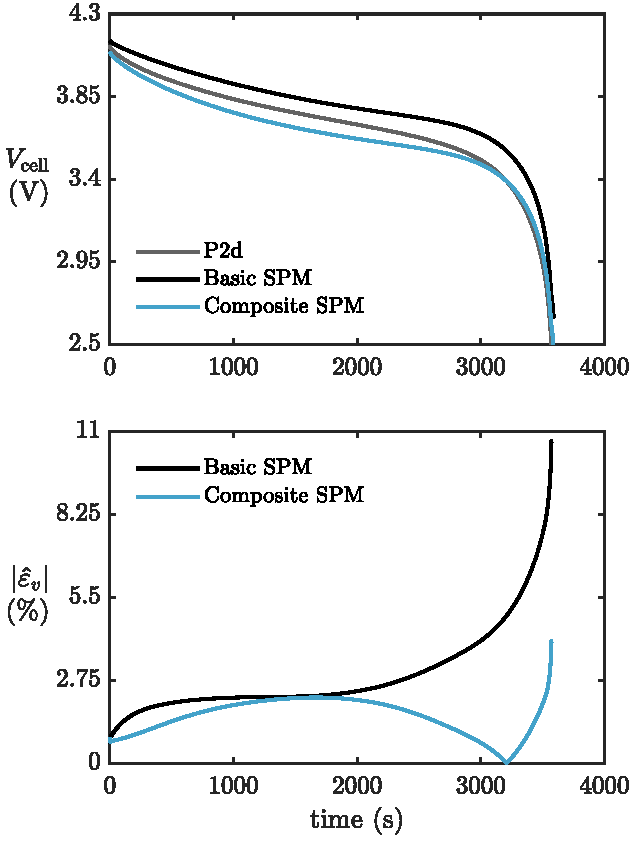
\includegraphics{composite_spm_vcell_1C.pdf}
    \caption[%
    Comparison  of  terminal  voltages  of  composite  \glsfmtshort{spm},  basic
    \glsfmtshort{spm} and the \glsfmtshort{p2d} model for a 1C~discharge
    ]%
    {%
        Voltage output  of various \glspl{spm}  for a 1C~discharge  beginning at
        \SI{100}{\percent} \gls{soc} (top  plot). Since it does  not account for
        electrolyte overpotentials,  the voltage  profile computed by  the basic
        \gls{spm} lies above that of the benchmark \gls{p2d} model. On the other
        hand, the composite \gls{spm} tends  to over correct for the electrolyte
        overpotential  so that  its terminal  voltage lies  below the  \gls{p2d}
        output. Since  the two \glspl{rom}  have outputs  on either side  of the
        \gls{p2d}  model,  it  is  convenient  to  use  the  absolute  error  to
        compare  them. In  the  bottom  plot, the  percentage  deviation of  the
        absolute error of the two  \glspl{rom} is shown. The composite \gls{spm}
        performs  significantly better  with a  peak absolute  error of  \approx
        \SI{4}{\percent} in  contrast to nearly \SI{11}{\percent}  for the basic
        \gls{spm}.
    }%
    \label{fig:voltageoutputcompareallSPMs1C}
\end{figure}

\Cref{fig:voltageoutputcompareallSPMs1C}  shows the  terminal voltage  output of
various \glspl{spm} for a 1C~discharge beginning at \SI{100}{\percent} \gls{soc}
(top  plot). Since  it  does  not account  for  electrolyte overpotentials,  the
voltage profile computed by the basic \gls{spm} lies above that of the benchmark
\gls{p2d}  model. On  the  other hand,  the composite  \gls{spm}  tends to  over
correct  for the  electrolyte overpotential  so that  its terminal  voltage lies
below  the \gls{p2d}  output. Since  the output  of the  two \glspl{rom}  lie on
either side of the \gls{p2d} model, it  is appropriate to use the absolute value
of their errors with respect to the  \gls{p2d} benchmark to compare them. In the
bottom  plot,  the  percentage  deviation  of the  absolute  error  of  the  two
\glspl{rom} is shown. The statistics of this deviation is quantified
in \cref{tbl:errorsummarycntcurrdischgallspms}.

% -*- root: ../main.tex -*-
%!TEX root = ../main.tex
% this file is called up by main.tex
% content in this file will be fed into the main document
% vim:textwidth=180 fo=cqt

\begin{table}[!htbp]
    \caption[%
    Summary of error statistics for basic \glsfmtshort{spm} and composite \glsfmtshort{spm} for 1C discharge
    ]%
    {%
    Summary of statistics for the percentage absolute error
        in terminal voltage
    for the basic \glsfmtshort{spm} and the composite \glsfmtshort{spm} in constant current 1C discharge simulations.
}%
    \label{tbl:errorsummarycntcurrdischgallspms}
    \centering
    \begin{tabular}{@{} l S[table-format=2.2] S[table-format=1.2] @{}}
        \toprule
        \makecell{Error Statistic \\ for \si{\percent}$\abs{\hat{\varepsilon}_v}$} & {\makecell{Basic \\ \glsfmtshort{spm}}} & {\makecell{Composite \\ \glsfmtshort{spm}}} \\
        \midrule
        %
        Worst Case        & 10.67 & 4.05 \\
        Mean              & 2.92  & 1.54 \\
        \glsfmtshort{rms} & 3.27  & 1.65 \\
        %
        \bottomrule
    \end{tabular}
\end{table}


In  each of  the error  statistic considered,  the composite  \gls{spm} performs
significantly better than the basic \gls{spm} for the 1C~discharge case.

One   of   the   biggest   drawbacks   of   the   conventional   \gls{spm}   was
its    poor    voltage    accuracy    at    moderate    C-rates    above~0.5C
(see \cref{tbl:errorsummarycntcurrdischgspmp2d}). The high accuracy achieved for
the 1C~rate  seems to indicate that  the composite \gls{spm} is  indeed a viable
solution for all  high C-rates, especially given the backdrop  of its methodical
derivation steeped in system identification.

However,  there exists  a  fundamental  flaw in  all  models  that use  a~priori
assumptions  of  simplified spatial  profiles  for  ionic concentration  in  the
electrolyte.  In  the  case  of  both the  baseline  quadratic  and  the  system
identification models, a parabolic profile spanning the entire thickness of each
region within the cell was chosen a~priori. However, no attempt to modify the
profile upon encountering an ion starvation event at any spatial location.

This  critical flaw  is  exposed  by the  sustained  application  of any  higher
current  that  induces  an  ion  starvation at  one  of  the  electrodes  during
operation. \Cref{fig:2Cionstarvation}  depicts  the  ionic concentration  in  the
electrolyte  over  time at  both  current  collectors  for a  2C~discharge.  The
profiles  computed  by  both  the \gls{p2d}  and  system  identification  models
are  plotted.  For  the  system  identification  model,  the  current  collector
interface  at  the  positive  electrode  experiences  an  ion  starvation  event
at~\approx\SI{150}{\second}. The  quadratic spatial  profile used by  this model
does not account for such a  reduction in the effective electrode thickness. All
the  boundary conditions  and coefficients  were formulated  using the  original
electrode  thickness.  Therefore,  beyond \SI{150}{\second},  the  concentration
becomes negative which  is not physically meaningful. The author  of this thesis
has implemented a saturation mechanism in the code that detects an ion depletion
event and prevents the concentrations from becoming negative.

Implementing  this  hard   lower  bound  of  zero  for   the  ion  concentration
does    not   mitigate    the   problems    associated   with    computing   the
electrolyte   overpotential.   Specifically,  computational   difficulties   are
encountered    when   computing    the    concentration   dependent    diffusion
overpotential \cref{eq:electrolytepdwithcenew}. In the case  of ion depletion at
the positive  current collector,  the argument of  the logarithmic  term becomes
zero which leads to a non-feasible computation~($-\infty$). Ion depletion at the
negative current collector  is equally detrimental to  the computation. However,
this scenario has  a lower probability owing to the  low C-rates during charging
operation (see \cref{subsec:basicspmsimsetup}).  Furthermore, in the  absence of
the lower  bound of zero  for the  concentrations, complex numbers  are obtained
from  the logarithmic  term, which  lead to  physically erroneous  overpotential
calculations. An  alternative is  to simply omit  the diffusion  impedance term.
However, since  this term is  responsible for  the large-signal dynamics  of the
overpotential (see \cref{fig:contributiontophiefromtwoterms}), omitting this and
reverting to  a simple ohmic  resistance contribution shall lead  to significant
errors  in  the electrolyte  overpotential,  and  consequently in  the  terminal
voltage.  Finally, setting  the diffusion  impedance to  zero at  the transition
boundary of ion starvation is also not a feasible solution. This is because, the
sudden inflection in  the trajectory of the terminal voltage  shall induce large
errors in any state estimation algorithms that depend on the composite \gls{spm}
as the plant model.

The  difficulties  encountered  in electrolyte  overpotential  computations  for
ion  depletion scenarios  have  not  yet been  discussed  in  the literature  by
the  research  community that  use  such  quadratic approximation  models.  This
thesis author  therefore assumes that  such a  scenario had not  been previously
encountered  for  the  parameter  set  and C-rate  combinations  used  by  those
researchers. Despite the  fact that this phenomenon might be  an artefact of the
idiosyncrasies of the  parameter set used here, it  is nevertheless questionable
to not  have mathematically adapted  the parabolic  profile to such  events. The
aspect  of rendering  the model  robust to  such vagaries  is currently  an open
problem in the field and can be the subject of future research. It can therefore
be concluded that  this composite \gls{spm} is \emph{unsuitable}  in its present
form for  sustained constant current  discharge at higher C-rates.  Despite this
setback due  to deficiencies in  the mathematical formulation of  the underlying
spatial profile, the superior performance  of the system identification model in
the computation  of ionic  concentrations and overpotentials  for \emph{dynamic}
conditions warrant such a study for the composite \gls{spm}.

\begin{figure}[!htbp]
    \centering
    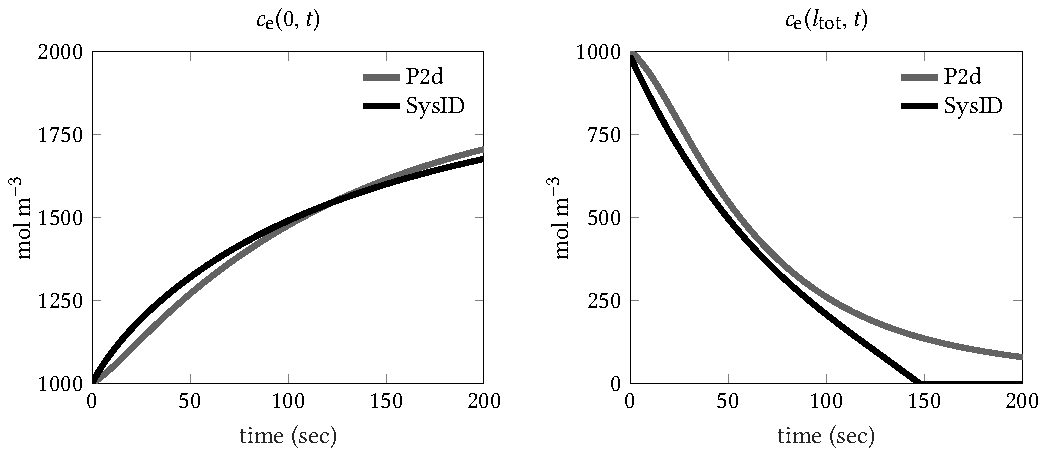
\includegraphics[width=\textwidth]{problematic_2C_conc.pdf}
    \caption[
    Time evolution of ionic concentration computed by the \glsfmtshort{p2d} and system
    identification models at both current collectors for a 2C~discharge
    ]
    {%
        Time evolution of ionic concentration in electrolyte computed by the \gls{p2d} and
        system identification models at ---
        \begin{enumerate*}[label=\emph{\alph*})]
            \item negative current collector interface (left plot), and
            \item positive current collector interface (right plot)
        \end{enumerate*}
        for a constant current discharge at \SI{120}{\ampere} \ie~2C. In the
        system identification mode, ion
        starvation occurs at the positive current collector interface at~\approx\SI{150}{\second}. The quadratic spatial profile used by the system
        identification model spans the entire electrode region and does not
        account for ion depletion scenarios. In this thesis, the author has
        implemented a saturation mechanism in the computer code to prevent the
        ionic concentration from becoming negative. Despite this
        mitigating action, the computation of electrolyte overpotential
        using \cref{eq:electrolytepdwithcenew} is problematic in such scenarios.
    }%
    \label{fig:2Cionstarvation}
\end{figure}

\subsubsection*{Dynamic Load Conditions}

In  order to  evaluate the  performance of  the composite  \gls{spm} to  dynamic
inputs, the  input profile  corresponding to  the \gls{udds}  drivecycle profile
in \cref{fig:uddssimp2dspmresults}  with  a  peak current  of  \SI{180}{\ampere}
\ie~3C was used.

\Cref{fig:voltageoutputcompareallSPMsudds}  shows  the  voltage  output  of  the
composite  \gls{spm}  for a  \gls{udds}  input  profile  with a  peak  magnitude
of   \SI{180}{\ampere}  \ie~3C  (see \cref{fig:uddssimp2dspmresults}).   The
voltage   profiles  computed   by  the   basic  \gls{spm}   and  the   benchmark
\gls{p2d}  model   is  also  overlaid   (top  plot).  The   percentage  absolute
error  of  the  two  \glspl{rom}  relative  to  the  \gls{p2d}  model  is  shown
in  the  bottom  plot.  Clearly,  it  is  seen  that  the  terminal  voltage  of
the  composite  \gls{spm}   is  significantly  more  accurate   than  the  basic
\gls{spm}  (see \cref{tbl:errorsummaryuddsdischgallspms}).   For  instance,  the
voltage  profile  computed by  composite  \gls{spm}  matches the  complex  shape
characteristics  of the  \gls{p2d} model  while remaining  very close  to it  in
magnitude.

\begin{figure}[!htbp]
    \centering
    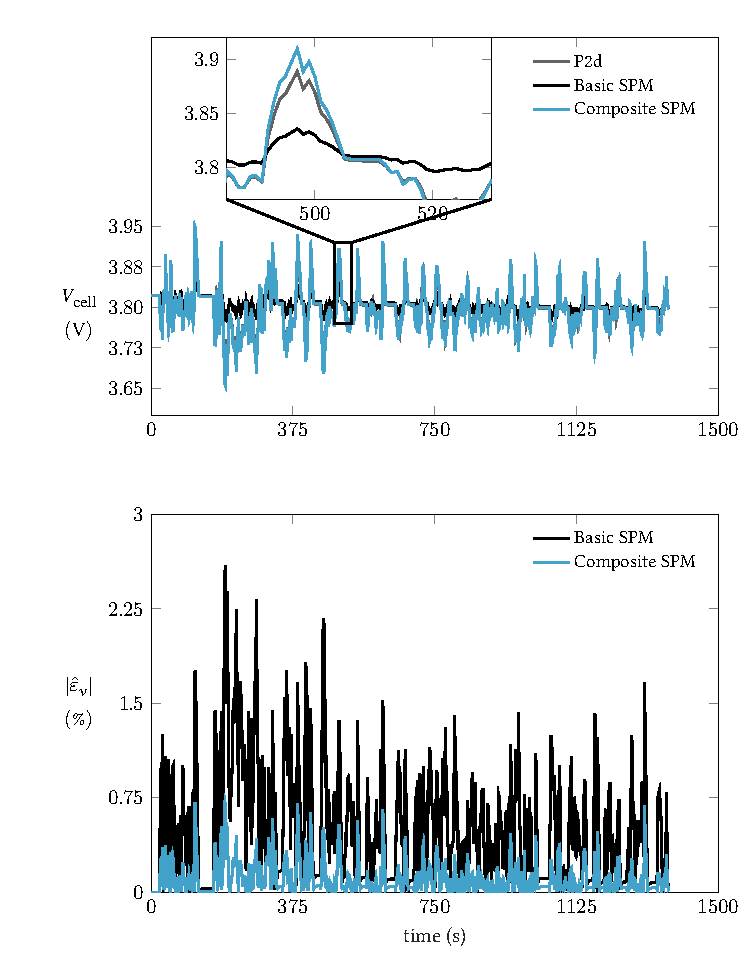
\includegraphics{composite_spm_vcell_udds.pdf}
    \caption[%
    Terminal voltage output of --- \emph{a}) the \glsfmtshort{p2d} model, \emph{b}) the
    basic \glsfmtshort{spm}, and \emph{c}) the composite \glsfmtshort{spm} for a
    \glsfmtshort{udds} input profile
    ]%
    {%
        Voltage output of the composite \gls{spm} for a \gls{udds} input profile
        with a peak magnitude of \SI{180}{\ampere} \ie~3C
        (see \cref{fig:uddssimp2dspmresults}). The voltage
        profiles computed by the basic \gls{spm} and the benchmark \gls{p2d}
        model is also overlaid (top plot). The percentage absolute error of the
        two \glspl{rom} relative to the \gls{p2d} model is shown in the bottom
        plot. The terminal voltage of the composite \gls{spm} is significantly
        more accurate than the basic \gls{spm}
        (see \cref{tbl:errorsummaryuddsdischgallspms}).
    }%
    \label{fig:voltageoutputcompareallSPMsudds}
\end{figure}

% -*- root: ../main.tex -*-
%!TEX root = ../main.tex
% this file is called up by main.tex
% content in this file will be fed into the main document
% vim:textwidth=180 fo=cqt

\begin{table}[!htbp]
    \caption[%
    Error statistics for basic  and composite \glsfmtshortpl{spm} for a \glsfmtshort{udds} load profile
    ]%
    {%
    Summary of statistics for the percentage absolute error
        in terminal voltage
        for the basic \glsfmtshort{spm} and the composite \glsfmtshort{spm} with \gls{udds} input profile.
}%
    \label{tbl:errorsummaryuddsdischgallspms}
    \centering
    \begin{tabular}{@{} l S[table-format=2.2] S[table-format=1.2] @{}}
        \toprule
        \makecell{Error Statistic \\ for \si{\percent}$\abs{\hat{\varepsilon}_v}$} & {\makecell{Basic \\ \glsfmtshort{spm}}} & {\makecell{Composite \\ \glsfmtshort{spm}}} \\
        \midrule
        %
        Worst Case        & 2.59 & 0.72 \\
        Mean              & 0.51 & 0.11 \\
        \glsfmtshort{rms} & 0.68 & 0.16 \\
        %
        \bottomrule
    \end{tabular}
\end{table}





% Conclude the chapter  by saying that everything is now  in time domain. Suitable
% for direct  implementation. Concludes the  implementation aspect of  the thesis.
% Can now be used as the plant model in EKF and other applications.

